Regression models are tools for understanding relationships between variables and predicting. However, for this to work, certain assumptions need to be satisfied. 
These assumptions are not guaranteed when working with data from real life, so how can we proceed with analyzing a regression model, if the method we use to make it, is not reliable?


\subsection{Assumptions for regression models}

\noindent This section will briefly explain the previously mentioned key assumptions that are needed to ensure reliable results, so the meaning behind them is clear.   \newline

\noindent The assumption independence of errors states that the errors from the model are not correlated with each other but are independent. This means that one error cannot be used to predict the next one. \newline


\noindent The assumption of linearity states that the relationship between the independent variables and the parameters, also known as the coefficients, is linear. This does not mean that the regression model itself has to be linear. For example, in polynomial regression, the relationship between the independent variables and the coefficients is still linear, but the independent variables can be transformed using powers.\newline


\noindent Homoscedasticity is the assumption of constant variance across errors for all levels of the independent variables. \newline

\noindent The assumption normality of errors states that the errors between the model and the observed values, also called residuals, are normally distributed. If this is not met, it may result in a biased model and a worse model fit. \newline


\noindent Multicollinearity occurs when two or more independent variables in a regression model are highly correlated with each other. This means that changes in one independent variable are associated with changes in another, making it difficult to determine the individual effect of each independent variable on the dependent variable. \newline

\noindent Correct model specifications assumes that the provided dependent variables for the models are the correct ones. If one is missing or the model is overfitting, this may result in incorrect coefficients and introduce errors into the model. \newline

\noindent Data does not always adhere to these assumptions, so the results may be inaccurate. 
If such a case occurs, there are different ways to accommodate the situation. These methods will be further discussed later on. \newline 

 

\subsubsection{Data from real-life}
An example of a data set containing violations in assumptions, specifically the assumptions of homscedasticity and no multicollinearity, is the "Miles Per Gallon" data set. Through the "Miles Per Gallon" it's possible to model the violations in the assumptions, as seen in \autoref{fig:1} and \autoref{fig:2}.
\newline

\begin{figure}
	\centering
	\centering
	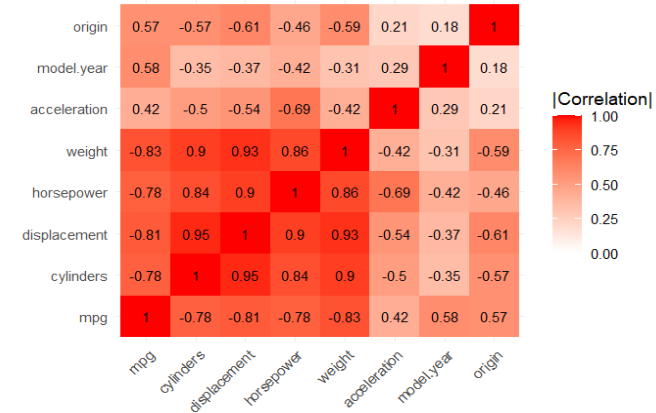
\includegraphics{billder/1.png}
	\caption{Heatmap made from the MPG dataset}
	\label{fig:1}
\end{figure}

\noindent Multicollinearity can be seen in Figure 1. Multicollinearit occurs when independent variables are highly correlated with each other, and as a result, it becomes more difficult to isolate the individual effect of each variable in a regression model.
In this model it is shown through the numbers, where the high numbers suggest a strong linear relationship through the variables. So between 'displacement' and ' cylinders', the value is 0.95, which is close to 1 and therefore shows there is multicollinearity. \newline

\begin{figure}[h]
	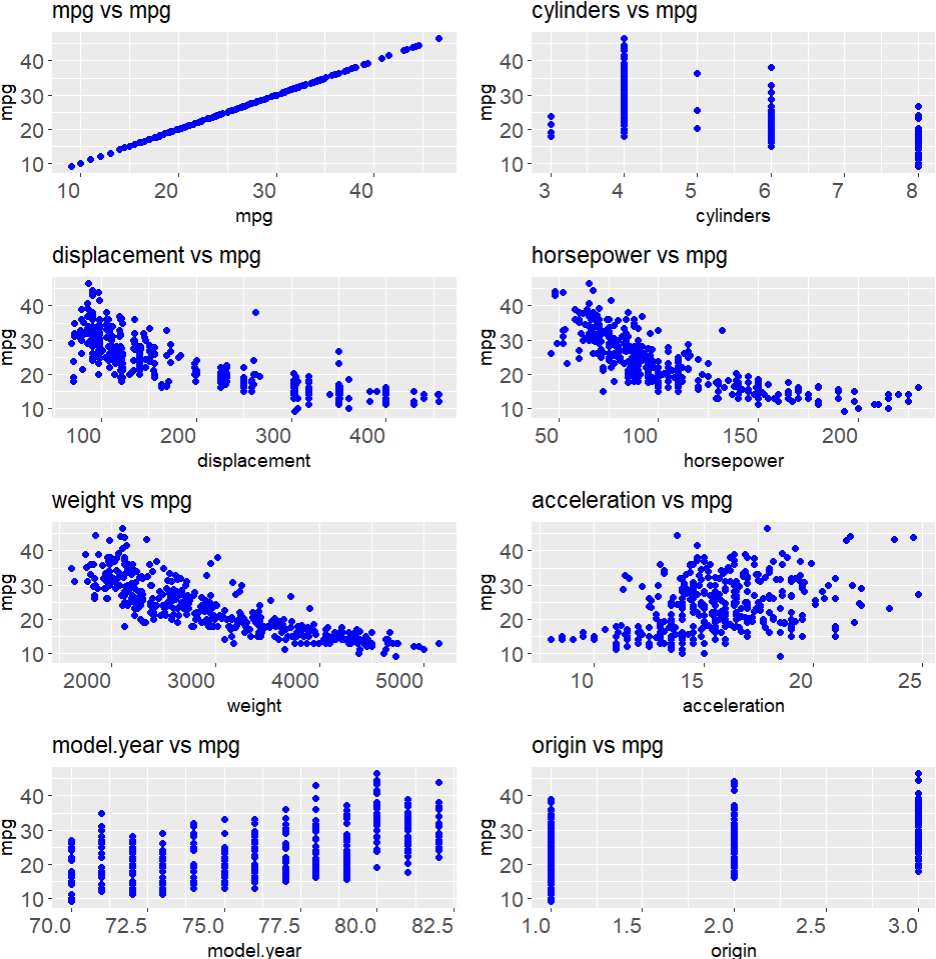
\includegraphics[width=\linewidth]{billder/2.png}
	\caption{Scatterplots made from the MPG dataset}
	\label{fig:2}
\end{figure}
There is an example of hetereoscedasticity in the 'mpg' and 'horsepower' scatterplot in Figure 2, where there is not constant variance of the residuals. This is seen because there is a big spread between the variables, especially when horsepower decreases.   

\noindent To understand how the classical method of constructing regression models and the method of using Monte Carlo Bootstrapping works, we need to dive deeper into the background. Here, we need to understand ways to not only create a model, but how to test it as well. These topics will be explained in the following section.

